\chapter[O Estudo de Caso]{O Estudo de Caso}


\section[A Organização]{A Organização}

O órgão escolhido, IPHAN, possui uma força de trabalho atuante na área de TI de apenas 8 funcionários, dos quais apenas 3 trabalham diretamente com sistemas. O perfil dessa equipe é apresentado na Tab. (3). Devido ao número reduzido de servidores disponíveis na área de TI do órgão, frequentemente uma mesma pessoa acaba desempenhando diferentes papeis requeridos pela Instrução Normativa MP/SLTI Nº04/2010.

\begin{table}[H]
\center
\footnotesize
\begin{tabular}{|c|c|c|}
\hline
\textbf{Área}          & \textbf{Perfil}   & \textbf{Quantidade} \\ \hline
TI Geral               & Coordenador de Tecnologia da Informação   & 1                   \\ \hline
Infraestrutura         & Analista de Tecnologia da Informação   & 2                   \\ \hline
Sistemas               & Analista de Tecnologia da Informação   & 2                   \\ \hline
\multirow{3}{*}{Apoio} & Analista de Tecnologia da Informação    & 1                   \\ \cline{2-3} 
\multicolumn{1}{|l|}{} & Servidor do Ministério da Ciência, Tecnologia e Inovação & 1                   \\ \cline{2-3} 
\multicolumn{1}{|l|}{} & Servidor do IPHAN & 1                   \\ \hline
\end{tabular}
\caption{Perfil da Equipe}
\end{table}

O contexto atual do órgão foi identificado por meio da aplicação da técnica de entrevista semi-estruturada. A estrutura da entrevista pode ser encontrada no Apêndice I -  Roteiro de Entrevista.

Os fatores mais significantes que são gerenciados pela área de TI do órgão, segundo o entrevistado, são:
\begin{itemize}
\item Atender as demandas para desenvolvimento de sistemas (sistema novo, manutenção, documentação).
\item Controlar de qualidade de sistemas.
\item Possuir medições de sistemas.
\end{itemize}

Por meio da entrevista foram identificados alguns problemas, dentre eles:
\begin{itemize}
\item Alguns contratos foram encerrados sem haver entrega de \textit{software};
\item Havia faturamento de Ordens de Serviço apenas com entrega de documentação;
\item Incapacidade de aferir a qualidade interna do produto;
\item As mudanças de requisitos geravam impacto no tempo de execução do projeto, ocasionando constantes atrasos.
\end{itemize}

A partir dos problemas identificados, ainda conforme o entrevistado, as principais motivações para o uso de metodologias ágeis na gestão de contratos foram: aumentar o volume de entregas \textit{software}; prover maior visibilidade do processo e do produto para o do gestor de negócio; empoderar o gestor do contrato sobre a gerência dos requisitos, de forma a eliminar  a interferência direta do gestor de contrato e, por fim, perceber de forma mais rápida se o projeto terá sucesso ou não, pois os riscos inerentes à contratação poderiam ser identificados com antecedência.

De acordo com a Instrução Normativa MP/SLTI Nº04/2010, a fase de Gerenciamento de Contrato deve conter as seguintes etapas: início do contrato; encaminhamento formal de ordem de serviço ou fornecimento de bens  monitoramento da execução; e transição contratual e/ou encerramento do contrato. Todas estas etapas podem estão contempladas no MIDAS, fazendo com que ele seja aderente ao normativo e adequado para o estudo de caso deste trabalho.

De acordo com o entrevistado, as metas norteadoras para a elaboração do MIDAS foram:
\begin{itemize}
\item Ser aderente à legislação pertinente;
\item Entregar \textit{software} mais rapidamente;
\item Focar na gestão do contrato e na definição de uma metodologia de gestão de demandas;
\item Não focar em dizer como a empresa deveria desenvolver o \textit{software}, ou seja, não definir metodologia de desenvolvimento de \textit{software};
\item Satisfazer as necessidades do cliente.
\end{itemize}

Outros instrumentos contratuais que foram modificados com o uso do MIDAS foram a forma de pagamento e a aplicação de multas. Em relação a esta, diferentemente das outras formas de gestão de contrato utilizadas anteriormente, onde as multas eram progressivamente aplicadas, por exemplo, sobre a não entrega de documentação somente além de deter caráter meramente punitivo. Com o MIDAS, passou-se a considerar o maturidade e crescimento da empresa no contrato e as multas eram somente aplicadas se não houvesse entrega de \textit{software}. O faturamento das ordens de serviço era executado a cada entrega, final de \textit{sprint}, com duração mensal, o que mantinha o fluxo de caixa da empresa contratada sempre ativo.

\section[Caracterização da Solução]{Caracterização da Solução}

Para desenvolver um modelo de contratação de fornecedores de \textit{software} baseado em Scrum e Kanban, o IPHAN definiu alguns procedimentos que deveriam ser feitos com o foco na minimização dos riscos da execução contratual e na obtenção do sucesso no contrato de terceirização. O \textit{framework} utilizado não é considerado o mais relevante, mas sim os valores e princípios do Manifesto Ágil, além do atendimento à legislação vigente. 

As metodologias ágeis foram utilizadas como o meio para atingir o sucesso ou para identificar de forma rápida os riscos iminentes. O sucesso contratual pode ser entendido como aquele contrato que atende às necessidades do órgão, com sistemas, sem comprometer o erário (tesouro público). Assim, para atingir sucesso em um contrato é preciso que pelos menos esses três procedimentos sejam realizados: \cite{parente}:
\begin{itemize}
\item Definir premissas nos artefatos desde o planejamento da contratação;
\item Alinhar diretrizes e condições com a Direção de TI;
\item Convalidar com a Alta Administração, ou seja, validar e sustentar essas diretrizes durante o contrato.
\end{itemize}

Com isso, foram definidas algumas premissas que devem orientar o planejamento e execução do contrato. A saber:  \cite{parente}:
\begin{itemize}
\item O órgão não deve definir, ou exigir, o uso de Metodologia Ágil da entidade contratada. Não defina Metodologia de Desenvolvimento de Software (MDS), mas sim a
forma de gerenciar as demandas (ordens de serviço), os produtos que devem ser entregues e seus critérios de aceitação. 
\item A recontagem de Pontos por Função nos moldes do roteiro do SISP com metodologia ágil que pode mudar constantemente é um risco. É preciso alterar o percentual definido para a alteração, manutenção ou refatoração de uma funcionalidade, definir corretamente o conceito de manutenção evolutiva, refatoração e alteração de requisito e evidenciar no processo o custo de uma alteração e fazer com que o gestor negocial, que pediu a alteração, assine a ordem de serviço e ateste a nota fiscal;
\item Só abra uma Ordem de Serviço (OS) por vez e por projeto. Pode-se ter várias OS abertas com a mesma Contratada, porém, será uma OS para cada projeto e uma OS por \textit{Sprint}; Além disso, nunca comece oficialmente a próxima demanda sem receber ou finalizar a demanda anterior. Caso uma OS não estiver atendendo o que foi solicitado, ou por uma mudança negocial essa OS não for necessária, cancele-a e abra outra ordem de serviço que atenda a nova exigência do gestor contratual;
\item Não gerencie atrasos ou defeitos. No fim da \textit{Sprint}, receba o que estiver pronto, mesmo que não seja tudo que foi solicitado. Se nada foi entregue é uma ausência de entrega, não existe atraso, a \textit{Sprint} é considerada perdida. O produto não entregue ou com defeito dever voltar para fila de demandas e entrará na próxima OS ou \textit{Sprint} se o gestor negocial a quiser novamente, nunca aceite que corrijam um produto com defeito dentro da mesma OS;
\item Entenda a demanda antes de executá-la. É preciso planejar, pelo menos, com quantas ordens de serviço o projeto será validado, qual o processo de negócio que será desenvolvido, como será feita a gestão de demandas e qual será a demanda da próxima \textit{Sprint} ou OS;
\item Não aceite documentos sem sistemas. É importante ter em mente que não deve-se aceitar entregas apenas de documentação sem um produto funcional;
\item Acredite na evolução da empresa. No começo, a empresa contratada poderá não conseguir entregar o que foi solicitado ou entregar um produto funcional, no entanto, progressivamente ela irá se adequar ao processo e evoluir. 
\end{itemize} 

Com essas premissas definidas o órgão construiu um Kanban para auxiliar a Gestão de Demandas. 

O Kanban definido pelo IPHAN possui quatro colunas ou raias e está ilustrado na Fig. (12).

\begin{figure}[H]
		\centering
		\label{fig05}
			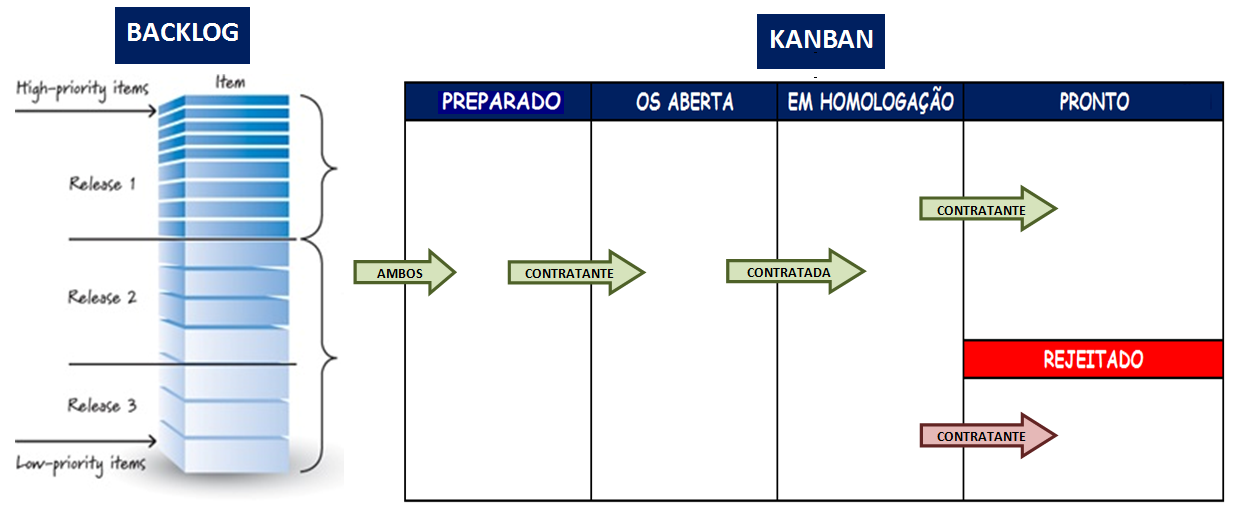
\includegraphics[scale=0.5]{figuras/kanbanIPHAN1.png}
		\caption{Quadro Kanban  \cite{parente}}
\end{figure}

A primeira raia do Kanban diz respeito aos itens que estão no estado “Preparado”. A condição de transição para esta raia pode ser feita da forma que o órgão quiser (Fig. 13). Por exemplo, os itens com mais prioridade podem ser os primeiros a irem para esta coluna. É importante que a definição de “Preparado” e a definição de “Pronto” estejam bem claras para todos os envolvidos.

\begin{figure}[H]
		\centering
		\label{fig06}
			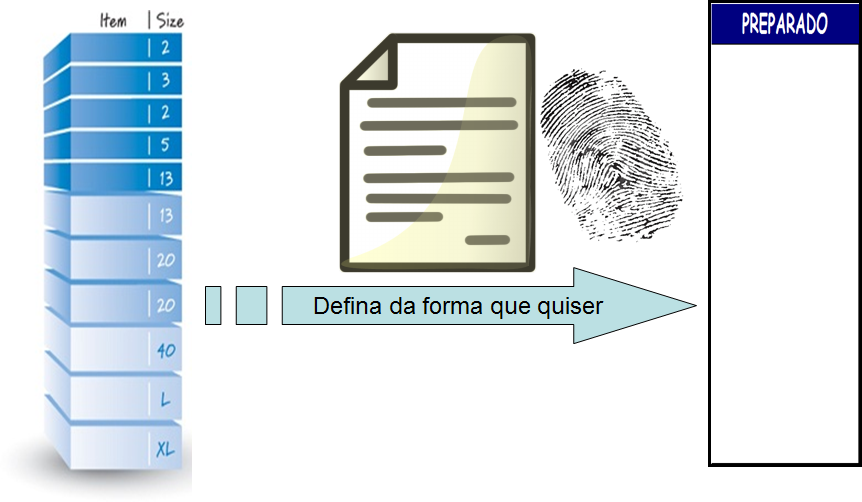
\includegraphics[scale=0.5]{figuras/kanbanIPHAN2.png}
		\caption{Transição para a raia Preparado \cite{parente}}
\end{figure}

A transição de um item da raia “Preparado” para a raia “OS Aberta” ocorre na abertura de uma ordem de serviço (Fig. 14). Ao observar o processo do MIDAS, percebe-se que essa transição ocorre após o planejamento da \textit{sprint}, no subprocesso \textit{Sprint}, onde uma ordem de serviço de desenvolvimento é aberta  com os itens que devem ser desenvolvidos para aquela \textit{sprint} e o desenvolvimento é iniciado. 

\begin{figure}[H]
		\centering
		\label{fig07}
			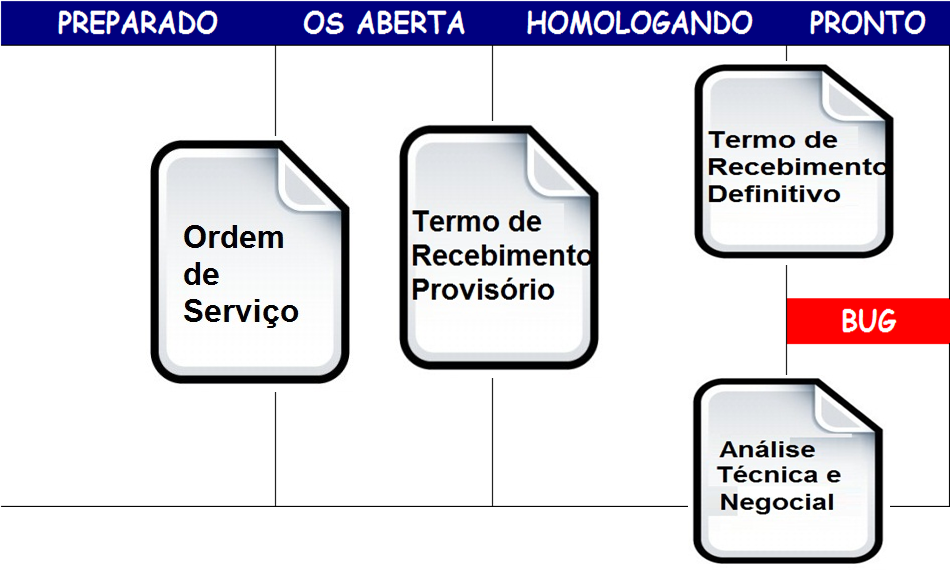
\includegraphics[scale=0.5]{figuras/kanbanIPHAN3.png}
		\caption{Transição entre raias \cite{parente}}
\end{figure}

A transição da raia “OS Aberta” para a raia “Homologando” ocorre quando o Termo de Recebimento Provisório é emitido (Fig. 14). Ao se observar o subprocesso de Realizar Ateste Técnico, percebe-se que essa transição ocorre na atividade “Receber Produtos”. Esta tem como entrada a ordem de serviço da fase e como saída o termo de recebimento provisório. Com a emissão do termo de recebimento provisório, os produtos recebidos entram na processo de homologação. 

A transição da raia “Homologando” para a raia “Pronto” ocorre quando o Termo de Recebimento Definitivo é emitido, ou seja, quando todos os produtos que foram anteriormente entregues são verificados e aprovados (Fig. 14). Para tanto são aferidos a aderência aos padrões técnicos e aos requisitos a partir de uma análise técnica e negocial, realizadas conjuntamente pelo Fiscal do Contrato e o Gestor de Negócio. Se forem detectados defeitos nos produtos entregues ou se eles forem rejeitados ou tiverem necessidade de refatoração, eles retornam para a fila de demandas, iniciando novamente o ciclo. A sinalização de rejeitado ou \textit{bug} diz respeito a funcionalidade que foi rejeitada por não atender o que foi pedido tanto funcionalmente quanto tecnicamente. A sinalização de refatoração diz respeito a mudança que é pedida em uma funcionalidade depois de ela já ter sido implementada. Para que uma funcionalidade entre nessa sinalização é preciso que o gestor de negócio assuma a responsabilidade pelos impactos que a mudança causará no custo, tempo e escopo.

Vale ressaltar que é importante que o trabalho em progresso (WIP) seja limitado conforme o que é conceituado no método Kanban. O IPHAN definiu um limite de 200 Pontos por Função por ciclo de trabalho (Fig. 15). 

\begin{figure}[h]
		\centering
		\label{fig08}
			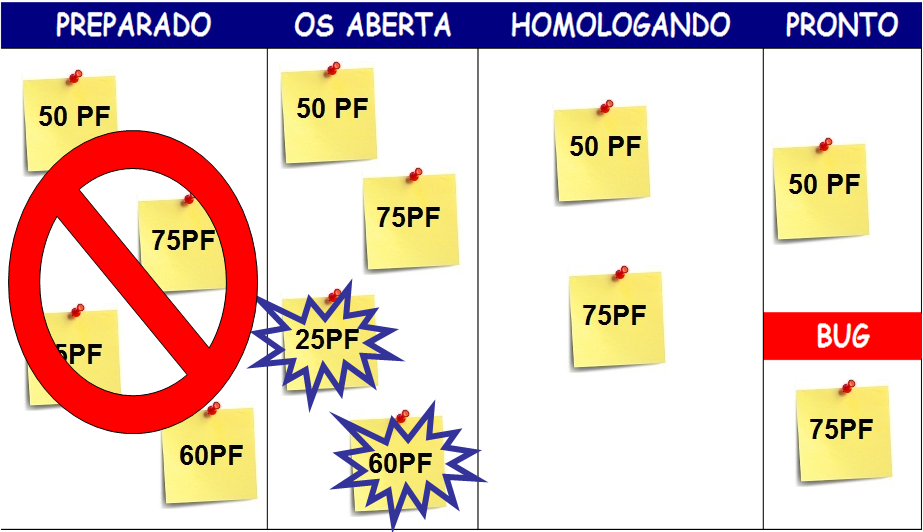
\includegraphics[scale=0.5]{figuras/kanbanIPHAN4.png}
		\caption{Limitação de WIP \cite{parente}}
\end{figure}

É importante sempre valorizar a entrega de produto funcional e não pagar por apenas documentação. Assim, o IPHAN dividia a forma de pagamento da contratada em percentuais, de acordo com a fase, valorizando a fase de execução, como ilustrado na Tab. (2).


\begin{table}[H]
\center
\footnotesize
\begin{tabular}{|p{6cm}|p{6cm}|}
  \hline
   \textbf{Fase} & \textbf{Percentual de Pagamento}\\
    \hline
   Planejamento (1 vez) & 5\%\\
   \hline    
   Execução (n vezes) & 80\%\\
    \hline
   Encerramento (1 vez) & 15\%\\
   \hline
\end{tabular}
\caption{Formas de Pagamento}
\end{table}


Outra técnica importante que foi construída diz respeito a parelização das atividades (Fig. 16). Enquanto uma ordem de serviço está na etapa de homologação, outra ordem de serviço pode ser preparada, evitando que o fluxo do processo pare e haja desperdício. 

\begin{figure}[H]
		\centering
		\label{fig09}
			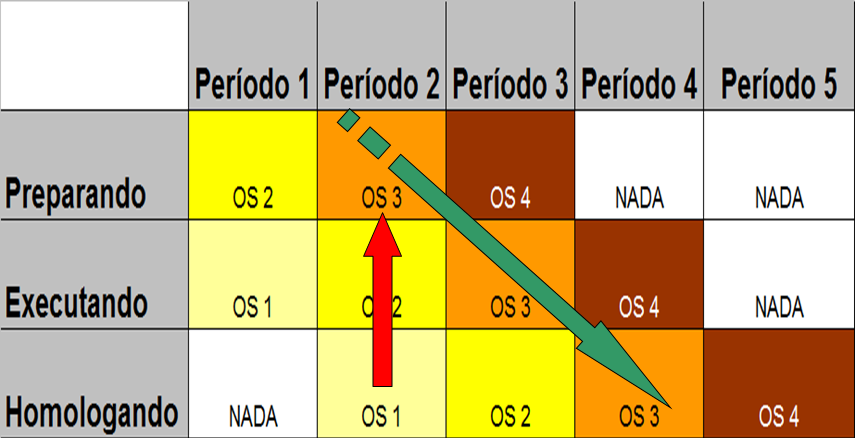
\includegraphics[scale=0.5]{figuras/kanbanIPHAN5.png}
		\caption{Parelização de Atividades \cite{parente}}
\end{figure}

O Kanban evidencia a aderência de utilização de métodos ágeis. A paralelização das atividades, que evita desperdícios de trabalho, evidencia a aderência ao Lean no Desenvolvimento de \textit{Software}. Assim, conclui-se que as premissas utilizadas como base para o desenvolvimento do Kanban foram baseadas tanto nos princípios ágeis quanto nos princípios do Lean. Após alguns meses de aplicação dessa solução o órgão deu início a construção da Metodologia IPHAN de Gestão de Demandas de Desenvolvimento Ágil de \textit{Software} (MIDAS). Uma parte do MIDAS pode ser visualizada no Anexo B. 


\section[Trabalho de Campo]{Trabalho de Campo}

\section[Caracterização do Contrato]{Caracterização do Contrato}


\section[Análise dos Dados]{Análise dos Dados}

\subsection[Efeitos sobre a entrega de ordens de serviço]{Efeitos sobre a entrega de ordens de serviço}

\subsection[Efeitos sobre a satisfação do cliente]{Efeitos sobre a satisfação do cliente}

\subsection[Efeitos sobre a qualidade do código]{Efeitos sobre a qualidade do código}


\section[Resultados]{Resultados}

